\documentclass[size=a4, parskip=half, titlepage=false, toc=flat, toc=bib, 12pt]{scrartcl}

% ---------------------------------------------------------------------------
%  PAQUETES
% ---------------------------------------------------------------------------

% IDIOMA
\usepackage[utf8]{inputenc}

% MATEMÁTICAS
\usepackage{amsmath}    % Paquete básico de matemáticas
\usepackage{amssymb}	% Fuentes matemáticas
\usepackage{mathtools}
%\usepackage{upgreek}
\usepackage{amsthm}     % Teoremas
\usepackage{mathrsfs}   % Fuente para ciertas letras utilizadas en matemáticas
\usepackage{bm}

\usepackage{tgpagella}  % text only
\usepackage{mathpazo}   % math & text


% LISTAS
\usepackage{enumitem}       % Mejores listas
\setlist{leftmargin=.5in}   % Especifica la indentación para las listas.

% Dibujos Tikz
\usepackage{pgf,tikz}
\usepackage{tkz-euclide}
%\usetkzobj{all}
\usepackage{mathrsfs}
\usetikzlibrary{arrows, calc,intersections,through,backgrounds}

% Títulos de figuras
\usepackage{capt-of}

% Posición de figuras
\usepackage{float}

% ---------------------------------------------------------------------------
%  RECURSOS
% ---------------------------------------------------------------------------

% Ruta donde buscar gráficos
\graphicspath{{../_assets/}, {_assets/}, {./img/}, {ALGI/img/}, {ALGI/}}

% ---------------------------------------------------------------------------
% ENTORNOS PERSONALIZADOS
% ---------------------------------------------------------------------------

%% DEFINICIONES DE LOS ESTILOS

% Nuevo estilo para definiciones
\newtheoremstyle{definition-style}  % Nombre del estilo
{}                                  % Espacio por encima
{}                                  % Espacio por debajo
{}                                  % Fuente del cuerpo
{}                                  % Identación
{\bfseries\tgpaella}                      % Fuente para la cabecera
{.}                                 % Puntuación tras la cabecera
{.5em}                              % Espacio tras la cabecera
{\thmname{#1}\thmnumber{ #2}\thmnote{ (#3)}}  % Especificación de la cabecera

% Nuevo estilo para notas
\newtheoremstyle{remark-style}
{10pt}
{10pt}
{}
{}
{\itshape \tgpaella}
{.}
{.5em}
{}

% Nuevo estilo para teoremas y proposiciones
\newtheoremstyle{theorem-style}
{}
{}
{}
{}
{\bfseries \tgpaella}
{.}
{.5em}
{\thmname{#1}\thmnumber{ #2}\thmnote{ (#3)}}

% Nuevo estilo para ejemplos
\newtheoremstyle{example-style}
{10pt}
{10pt}
{}
{}
{\bfseries \tgpaella}
{}
{.5em}
{\thmname{#1}\thmnumber{ #2.}\thmnote{ #3.}}

% Nuevo estilo para la demostración

\makeatletter
\renewenvironment{proof}[1][\proofname] {\par\pushQED{\qed}\normalfont\topsep6\p@\@plus6\p@\relax\trivlist\item[\hskip\labelsep\itshape\tgpaella#1\@addpunct{.}]\ignorespaces}{\popQED\endtrivlist\@endpefalse}
\makeatother

%% ASIGNACIÓN DE LOS ESTILOS

% Teoremas, proposiciones y corolarios
\theoremstyle{theorem-style}
\newtheorem{nth}{Teorema}[section]
\newtheorem{nprop}{Proposición}[section]
\newtheorem{ncor}{Corolario}[section]
\newtheorem{nlema}{Lema}[section]

% Definiciones
\theoremstyle{definition-style}
\newtheorem{ndef}{Definición}[section]

% Notas
\theoremstyle{remark-style}
\newtheorem*{nota}{Nota}

% Ejemplos
\theoremstyle{example-style}
\newtheorem{ejemplo}{Ejemplo}[section]

% Ejercicios y solución
\theoremstyle{definition-style}
\newtheorem{ejer}{Ejercicio}[section]

\theoremstyle{remark-style}
\newtheorem*{sol}{Solución}

% ---------------------------------------------------------------------------
% COMANDOS PERSONALIZADOS
% ---------------------------------------------------------------------------

% Números enteros: \ent
\providecommand{\ent}{\mathbb{Z}}

% Números racionales: \rac
\providecommand{\rac}{\mathbb{Q}}

% Números naturales: \nat
\providecommand{\nat}{\mathbb{N}}


% Valor absoluto: \abs{}
\providecommand{\abs}[1]{\lvert#1\rvert}

% Fracción grande: \ddfrac{}{}
\newcommand\ddfrac[2]{\frac{\displaystyle #1}{\displaystyle #2}}

% Texto en negrita en modo matemática: \bm{}
\newcommand{\bm}[1]{\boldsymbol{#1}}

% Línea horizontal.
\newcommand{\horrule}[1]{\rule{\linewidth}{#1}}

% Restricción de una aplicación.
\newcommand\restr[2]{{% we make the whole thing an ordinary symbol
  \left.\kern-\nulldelimiterspace % automatically resize the bar with \right
  #1 % the function
  \vphantom{\big|} % pretend it's a little taller at normal size
  \right|_{#2} % this is the delimiter
  }}

% Imagen de una aplicación.
\DeclareMathOperator*{\img}{img}

% Divisores de un elemento de un anillo
\DeclareMathOperator*{\rdiv}{div}

% Listas ordenadas con números romanos (i), (ii), etc.
\newenvironment{nlist}
{\begin{enumerate}
    \renewcommand\labelenumi{(\emph{\roman{enumi})}}}
  {\end{enumerate}}

% División por casos con llave a la derecha.
\newenvironment{rcases}
{\left.\begin{aligned}}
    {\end{aligned}\right\rbrace}


% ---------------------------------------------------------------------------
%  COLORES
% ---------------------------------------------------------------------------

\usepackage{xcolor}     % Permite definir y utilizar colores

\definecolor{50}{HTML}{FFEBEE}
\definecolor{300}{HTML}{E57373}
\definecolor{500}{HTML}{F44336}
\definecolor{700}{HTML}{D32F2F}
\definecolor{900}{HTML}{B71C1C}


\setuptoc{toc}{leveldown}

% Ajuste de las líneas y párrafos
\linespread{1.2}
\setlength{\parindent}{0pt}
\setlength{\parskip}{12pt}

% Español
\usepackage[spanish, es-tabla]{babel}

% Matemáticas
\usepackage{amsmath}
\usepackage{amsthm}

% Links
%\usepackage{hyperref}

% Fuentes
%\usepackage{newpxtext,newpxmath}
\usepackage[scale=.9]{FiraMono}
\usepackage{FiraSans}
\usepackage[T1]{fontenc}

\defaultfontfeatures{Ligatures=TeX,Numbers=Lining}
\usepackage[activate={true,nocompatibility},final,tracking=true,factor=1100,stretch=10,shrink=10]{microtype}
\SetTracking{encoding={*}, shape=sc}{0}

\usepackage{graphicx}
\usepackage{float}

% Mejores tablas
\usepackage{booktabs}

\usepackage{adjustbox}

% COLORES

\usepackage{xcolor}

\definecolor{verde}{HTML}{007D51}
\definecolor{esmeralda}{HTML}{045D56}
\definecolor{salmon}{HTML}{FF6859}
\definecolor{amarillo}{HTML}{FFAC12}
\definecolor{morado}{HTML}{A932FF}
\definecolor{azul}{HTML}{0082FB}
\definecolor{error}{HTML}{b00020}

% ENTORNOS
\usepackage[skins, listings, theorems]{tcolorbox}

\newtcolorbox{recuerda}{
  enhanced,
%  sharp corners,
  frame hidden,
  colback=black!10,
	lefttitle=0pt,
  coltitle=black,
  fonttitle=\bfseries\tgpaella\scshape,
  titlerule=0.8mm,
  titlerule style=black,
  title=\raisebox{-0.6ex}{\small RECUERDA}
}

\newtcolorbox{nota}{
  enhanced,
%  sharp corners,
  frame hidden,
  colback=black!10,
	lefttitle=0pt,
  coltitle=black,
  fonttitle=\bfseries\tgpaella\scshape,
  titlerule=0.8mm,
  titlerule style=black,
  title=\raisebox{-0.6ex}{\small NOTA}
}

\newtcolorbox{error}{
  enhanced,
%  sharp corners,
  frame hidden,
  colback=error!10,
	lefttitle=0pt,
  coltitle=error,
  fonttitle=\bfseries\tgpaella\scshape,
  titlerule=0.8mm,
  titlerule style=error,
  title=\raisebox{-0.6ex}{\small ERROR}
}

\newtcblisting{shell}{
  enhanced,
  colback=black!10,
  colupper=black,
  frame hidden,
  opacityback=0,
  coltitle=black,
  fonttitle=\bfseries\tgpaella\scshape,
  %titlerule=0.8mm,
  %titlerule style=black,
  %title=Consola,
  listing only,
  listing options={
    style=tcblatex,
    language=sh,
    breaklines=true,
    postbreak=\mbox{\textcolor{black}{$\hookrightarrow$}\space},
    emph={jmml@UbuntuServer, jmml@CentOS},
    emphstyle={\bfseries},
  },
}

\newtcbtheorem[number within=section]{teor}{\small TEOREMA}{
  enhanced,
  sharp corners,
  frame hidden,
  colback=white,
  coltitle=black,
  fonttitle=\bfseries\tgpaella,
  %separator sign=\raisebox{-0.65ex}{\Large\MI\symbol{58828}},
  description font=\itshape
}{teor}

\newtcbtheorem[number within=section]{prop}{\small PROPOSICIÓN}{
  enhanced,
  sharp corners,
  frame hidden,
  colback=white,
  coltitle=black,
  fonttitle=\bfseries\tgpaella,
  %separator sign=\raisebox{-0.65ex}{\Large\MI\symbol{58828}},
  description font=\itshape
}{prop}

\newtcbtheorem[number within=section]{cor}{\small COROLARIO}{
  enhanced,
  sharp corners,
  frame hidden,
  colback=white,
  coltitle=black,
  fonttitle=\bfseries\tgpaella,
  %separator sign=\raisebox{-0.65ex}{\Large\MI\symbol{58828}},
  description font=\itshape
}{cor}

\newtcbtheorem[number within=section]{defi}{\small DEFINICIÓN}{
  enhanced,
  sharp corners,
  frame hidden,
  colback=white,
  coltitle=black,
  fonttitle=\bfseries\tgpaella,
  %separator sign=\raisebox{-0.65ex}{\Large\MI\symbol{58828}},
  description font=\itshape
}{defi}

\newtcbtheorem{ejer}{\small EJERCICIO}{
  enhanced,
  sharp corners,
  frame hidden,
  left=0mm,
  right=0mm,
  colback=white,
  coltitle=black,
  fonttitle=\bfseries\tgpaella,
  %separator sign=\raisebox{-0.65ex}{\Large\MI\symbol{58828}},
  description font=\itshape,
  nameref/.style={},
}{ejer}

% CÓDIGO
\usepackage{listings}

% CABECERAS
\pagestyle{headings}
\setkomafont{pageheadfoot}{\normalfont\normalcolor\tgpaella\small}
\setkomafont{pagenumber}{\normalfont\tgpaella}

% ALGORITMOS
\usepackage[vlined,linesnumbered]{algorithm2e}

% Formato de los pies de figura
\setkomafont{captionlabel}{\scshape}
\SetAlCapFnt{\normalfont\scshape}
\SetAlgorithmName{Algoritmo}{Algoritmo}{Lista de algoritmos}

% BIBLIOGRAFÍA
%\usepackage[sorting=none]{biblatex}
%\addbibresource{bibliografia.bib}

% REFERENCIAS
\usepackage[bookmarks = true, colorlinks=true, linkcolor = black, citecolor = black, menucolor = black, urlcolor = black]{hyperref}

\begin{document}

\renewcommand{\proofname}{\normalfont\tgpaella\bfseries\small DEMOSTRACIÓN}

\title{Método de ranking en el diseño de un sistema de acceso a la información}
\subject{Trabajo fin de grado}
\author{Johanna Capote Robayna\\
    Doble Grado en Ingeniería Informática y Matemáticas}
\date{}
\publishers{\vspace{2cm}
\includegraphics[height=2.5cm]{UGR}\vspace{1cm}}
\maketitle

\newpage

\tableofcontents
\newpage

\section{Introducción}
Fue en la década de los 80 cuando Internet empieza a darse a conocer con unas primeras páginas web de estilo muy básico y sencillo que tardaban mucho en cargarse. Con el transcurso del tiempo la Red fue creciendo a pasos agigantados almacenando un gran volumen de información lo que provocó  un sinfín de procesos y cambios en las formas de gestionarla, y es en ese contexto donde surgen los buscadores para dar respuesta a la necesidad de clasificar y gestionar gran cantidad de información lo más rápido posible.

Un buscador o motor de búsqueda es un sistema de recuperación de información, donde el usuario introduce una serie de términos o palabras clave y el buscador le devuelve una lista de resultados ordenados bajo una serie de criterios. WebCrawler, Lycos, AltaVista o Yahoo entre otros, son los primeros buscadores de la Historia que funcionaban de una forma muy similar, rastreaban la Red y clasificaban las páginas en función de las veces que contenían las palabras clave introducidas. Eran los más utilizados en esa época hasta que en 1998 son desbancados por Google, el mayor motor de búsqueda de todos los tiempos,  que consigue imponerse al resto de buscadores gracias a un nuevo algoritmo de búsqueda (PageRank), capaz de ordenar una gran cantidad de información en poco tiempo.

PageRank, es un algoritmo basado en el Álgebra lineal, Teoría de Grafos y Probabilidad, fue diseñado por Sergey Brin y Lawrence Page, el primero graduado en Matemáticas y el segundo en Informática y ambos estudiantes de doctorado de Informática de la Universidad de Standford. La pregunta que buscaban resolver era clara ``?`en qué orden mostrar los resultados de la búsqueda?''. En 1997 cuando Brin y Page empezaron a trabajar en el diseño del algoritmo se plantearon como objetivo principal que en el gran número de los casos, al menos una de las primeras páginas que se muestran como resultado contenga información útil para el usuario. Hay que tener en cuenta que en esta época Internet no era tan grande como ahora, habían censadas en torno a 100 millones de páginas web y los buscadores más famosos de la época eran capaces de atender 20 millones de consultas al día, mientras que hoy en día Google es capaz de atender a 200 millones de consultas diarias. Pasaremos a explicar cómo el algoritmo de PageRank es capaz de ordenar estas millones de páginas web en tan poco tiempo.

\section{Introducción al modelo}
Lo primero que hace Google, incluso antes de que el usuario realice la búsqueda es organizar el contenido de Internet ayudándose de un índice. Este índice se va actualizando y va añadiendo páginas nuevas y modificando la información de las páginas ya existentes en un proceso llamado ``rastreo'', en el cual adquiere información de esas páginas incluyendo los enlaces hacia otra páginas. El índice se ordena con el algoritmo de \textbf{PageRank}, el cual se explicará a continuación, que ordena la lista asignando un PageRank más alto a las páginas que calificará de ``más interesantes'' y un PageRank bajo a las páginas ``menos interesantes''.

Una vez que el usuario introduce su búsqueda esta pasa por varias fases:
\begin{itemize}
\item Análisis de las palabras del usuario. En esta fase se busca entender el significado de la búsqueda, para ello se analiza las palabras usadas y se interpreta lo que el usuario quiere decir con ellas. Este proceso incluye varios pasos como \textbf{interpretar los errores de ortografía} o entender el significado que el usuario le está dando a una palabra con varias acepciones ayudándose de un \textbf{sistema de sinónimos}. Otro aspecto importante de esta fase es el \textbf{algoritmo de novedades}, el cual deduce que en ciertas búsquedas debe mostrar la información más actual, como por ejemplo si el usuario busca ``horóscopo'' o ``resultados del fútbol club Granada'' se está interesando por las últimas publicaciones.
\item Búsqueda de coincidencias. En esta fase se busca entre las páginas del índice aquellas con información coincidente con la búsqueda. Se analiza la frecuencia con la que aparecen las palabras introducidas en las páginas web candidatas y su localización; es decir, si aparecen en el título, encabezamientos o en el cuerpo del texto. Además existen otros algoritmos que analizan si las páginas candidatas pueden resultar interesantes para el usuario, ya que si por ejemplo el usuario busca ``pájaros'' lo más probable es que no quiera encontrar una página con poca información relevante sobre el tema pero en la que se repite muchas veces la palabra ``pájaro''.
\item Mejora del posicionamiento de las páginas útiles. Una vez obtenidas las páginas web con información potencialmente válida se pasa a clasificar su utilidad con el objetivo de mostrar primero las páginas más útiles para el usuario. En esta fase se analizan varios factores como el número de veces que aparece el término buscado en la página, la fecha de publicación y la calidad de experiencia del usuario en la página. Además se descartan aquellos sitios web con contenido fraudulento o \textit{spam} y se potencia las páginas que en consultas similares hayan sido fiables.
\item Devolver los mejores resultados. En esta parte se busca la diversidad de respuestas. Antes de mostrar el resultado de la búsqueda se analiza el resultado en conjunto, se evalúa si hay muchas páginas centradas en la misma interpretación de la búsqueda o si solo existe un tema en los resultados.
\item Análisis del contexto. Esta fase no se realiza siempre, en ella se busca ``personalizar'' la búsqueda con datos como la ubicación o historial de búsqueda. Con ello se consigue reducir la búsqueda a su entorno, por ejemplo si el usuario es español y busca ``baloncesto'' le saldrá antes información sobre el baloncesto en España que sobre el de otros países o si el usuario busca ``conciertos cerca de mi'' aparecerán los conciertos más cercanos a su residencia. Además mediante el historial de búsqueda personal el buscador consigue mejorar la interpretación de la búsqueda, por ejemplo si el usuario ha buscado anteriormente ``Granada vs Osasuna'' y más adelante busca ``Granada'' puede considerar que el usuario se refiere al equipo de fútbol y no a la ciudad.
\end{itemize}

\newpage

\section{Descripción del problema}
El problema que se va a abordar en este trabajo es conseguir un método de \textit{ranking} para ordenar la información según el interés del usuario. Para ello se investigarán las ténicas utilizadas por uno de los mayores motores de búsqueda, Google, y se aplicarán sobre la base de datos PMSC-UGR. Para abordar el problema nos centramos en la parte preliminar a una búsqueda. Como ya se comentó anteriormente, antes de que el usuario realice una búsqueda en Google las páginas web ya se encuentran previamente ordenadas por el algoritmo PageRank. Este algoritmo  es en el que se centrará este trabajo dividido en dos grandes partes:
\begin{itemize}
\item En la primera parte se realizará un estudio teórico del algoritmo PageRank, en el que se datallará la base matemática de manera formal. En primer lugar se ajustara nuestro problema a un problema de valores y vectores propios y a continuación se desarrollaran varios resultados matemáticos que garantizan la existencia de una solución.
\item En la segunda parte se realizará un estudio práctico sobre el algoritmo PageRank sobre una base de datos y a continuación (... ??)
\end{itemize}

\section{Planificación}
Hacer diagrama de Grannt cada 2 o 3 semanas.

\newpage

\part{Matemáticas}

\section{Modelo matemático}

El algoritmo de PageRank utilizado para ordenar las páginas web tiene una base matemática de Álgebra Lineal: transformaremos el problema de ordenar las páginas web según su interés en un problema clásico de valores propios y vectores propios.

En primer lugar, vamos a definir el marco donde nos encontramos. Nuestro problema actual es establecer un criterio para ordenar las páginas de la red. Si llamamos $P_1, \dots, P_n$ a cada una de las páginas, siendo $n$ un número natural ($n \in \mathbb{N}$), definimos entonces la importancia $x_i$  de la página $P_i$ como un número real entre $0$ y $1$.

Esta importancia la utilizaremos para elegir qué páginas web son las primeras que mostramos en el buscador, ordenándolas de mayor  a menor valor de importancia.
Para calcular este número nos basamos en la información que podemos extraer de la red (sitios, contenido, enlaces de una página web a otra, etc).

En el primer modelo nos quedamos solo con los enlaces entre páginas web. Estos enlaces los podemos representar mediante un grafo dirigido (G), en el cual representamos cada $P_i$ como un nodo del grafo y por cada enlace de una página $P_i$ a $P_j$ añadimos una arista de $P_j$ a $P_i$ indicando el final con una punta de flecha, como se muestra en la imagen.

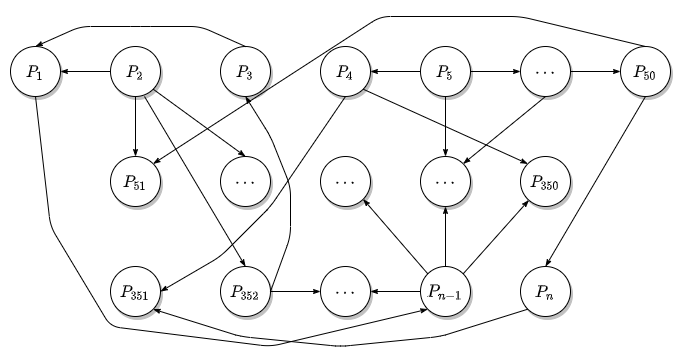
\includegraphics[width=1.0\textwidth]{./img/grafogrande}

Esta información la podemos reflejar en una matriz M de dimensión $nxn$. Tanto en las filas como en las columnas representamos las $n$ páginas y por cada enlace entre una página $j$ a otra página $i$, escribimos un $1$ en la entrada de la
matriz $m_{ij}$ y en el caso de que no haya enlace escribimos un $0$.

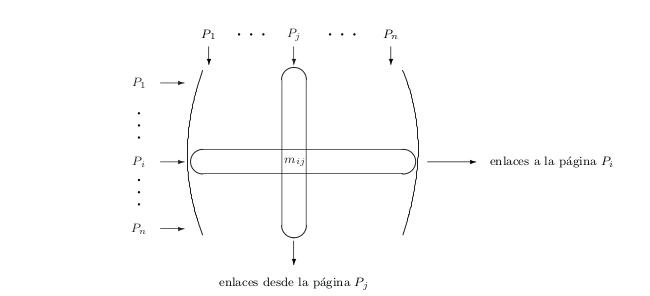
\includegraphics[width=1.0\textwidth]{./img/matriz}

Por lo tanto en la columna $j$ estarán los enlaces que salen de la página $P_j$ hacia otras páginas
mientras que en la fila $i$ estarán representados los enlaces a la página $P_i$. Esta matriz
no es simétrica ya que una página puede estar citada por otra y ella no citar a ninguna.

En una primera aproximación de querer ordenar las páginas web por ``importancia'' o ``relevancia'' podemos pensar que la página a la que le lleguen más enlaces (fila con mayor número de $1$) es la que debería mostrarse primero en el \textit{ranking}. Es decir si $x_j$ es la importancia de $P_j$, esta es proporcional al número de páginas desde las que hay enlaces a $P_j$.

Sin embargo, la realidad es que el número de enlaces a una cierta página no representa del todo su importancia, ya que no es lo mismo que esta esté citada por una página cualquiera a que esté citada desde \verb|www.facebook.com| o \verb|www.apple.com|. Estos dos últimos enlaces deberían ponderar más en importancia que otras citas de otras páginas web menos relevantes. Por lo que para asignar importancia a una página web, deberemos tener en cuenta tanto si es una \textbf{página muy citada} como si es una \textbf{página poco citada, pero de sitio ``relevantes''}.

Nos damos cuenta de que la importancia de la página citadora también es relevante, por lo que en una segunda aproximación pasamos a decidir que la importancia $x_j$ de una página $P_j$ es proporcional a la suma de las importancias de las páginas que enlazan con $P_j$. El cambio reside en que en la primera aproximación del modelo la importancia de $P_i$ era proporcional al número de páginas que enlazan con $P_i$, mientras que en esta segunda aproximación la importancia de $P_i$ es proporcional a la suma de las importancias de las páginas que enlazan con $P_i$.

Supongamos, por ejemplo, que la página $P_1$ es citada desde las páginas $P_{200}$ y $P_{n}$ ,
 que $P_2$ se cita desde $P_1$ , $P_{50}$ , $P_{200}$ y $P_n$ , mientas que en la última página $P_n$ hay enlaces desde $P_1$ , $P_2$ , $P_{50}$ , $P_{200}$ y $P_{n-1}$. En nuestra asignación anterior, $x_1, \dots , x_n$ deberían
 cumplir entonces que:
 $$ x_1 = K (x_{200} + x_n) $$
 $$ x_2 = K (x_{50} + x_{200} + x_{n-1}) $$
 $$ \vdots $$
 $$x_n = K (x_1 + x_2 + x_{50} + x_{200} + x_{n-1}) $$

donde $K$ es una constante de proporcionalidad. Si nos fijamos, hemos construido un sistema de ecuaciones
donde las soluciones son los posibles valores de $x_1, \dots , x_n$. Este sistema de ecuaciones
lo podemos escribir en términos matriciales:

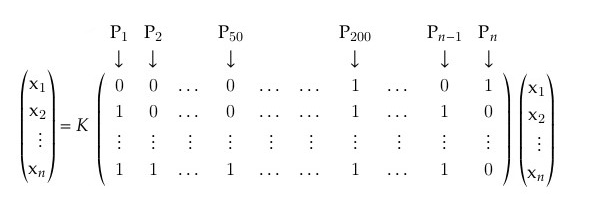
\includegraphics[width=1.0\textwidth]{./img/matrizejemplo}
%% TODO: cambiar plantilla
Si llamamos $\vec{x}$ al vector de importacias $(x_1 \dots x_n)$, $\lambda = \frac{1}{K}$ y
$M$ a la matriz de dimensiones $n x n$ del sistema (matriz asociada al grafo). Nos encontramos
con un problema de valores propios y vectores propios:
$$M \vec{x} = \lambda \vec{x} $$

A este vector $\vec{x}$ le exigimos que sea no negativo, es decir, que todas sus componentes sean no negativas, ya que representa la importancia de una página web y también buscamos que sea ``único'', en el sentido de que cualquier otro vector propio asociado a ese mismo valor propio sea múltiplo de este, ya que como nuestro objetivo final es establecer un \textit{ranking}, de haber dos vectores linealmente independientes tendríamos dos formas distintas de ordenar y habría que diseñar otro proceso de selección.

El estudio de la existencia de vector propio con esas propiedades para matrices con todas sus entradas no negativas es el objetivo de la Teoría de Perron-Frobenius que desarrollaremos en la siguiente sección.

\newpage

\section{Teorema de Perron-Frobenius}

Como hemos dicho anteriormente, en esta sección nos centraremos en el Teorema de Perron-Frobenius. Este resultado garantiza la existencia de un valor propio cumpliendo las propiedades que son la base del algoritmo del Pagerank.

Todos los resultados aquí expuestos se pueden encontrar, por ejemplo, en \cite{algebralineal}.

En primer lugar pasamos a introducir algunas notaciones y definiciones que usaremos posteriormente.

Dadas $A = (a_{ij}),B = (b_{ij}) \in M_n(\mathbb{C})$ y $\vec{x} = (x_1, \dots, x_n)^t\in \mathbb{C}^n$:
\begin{enumerate}
\item Diremos que $A$ es no negativa si $a_{ij}\geq 0$ , $1 \leq i,j \leq n$ y lo notaremos
$A\geq 0$.
\item Diremos que $A$ es positiva si $a_{ij} > 0$ , $1 \leq i, j \leq n$ y lo notaremos $A > 0$.
\item Diremos que $B$ es mayor o igual que $A$ si $a_{ij} \leq b_{ij}$, $1 \leq i,j \leq n$ y lo notaremos $A \leq B$.
\item Diremos que el vector $\vec{x}$ es no negativo si $x_i \geq 0$ , $1 \leq i \leq n$ y lo notaremos $\vec{x} \geq 0$.
\item Análogamente diremos que el vector $\vec{x}$ es positivo si $x_i > 0$, $1 \leq i \leq n$ y lo notaremos $\vec{x} > 0$.
\end{enumerate}

Denotaremos, como es habitual:
\begin{enumerate}
\item $\sigma (A)$ al espectro de $A$, es decir $\sigma(A) = \{ \lambda \in \mathbb{C} : det(A - \lambda I)= 0\}$
\item $\rho(A)$ al radio espectral de $A$, es decir $\rho(A) = \max\{|\lambda| : \lambda \in \sigma(A) \}$.
\item $m(\lambda)$ a la multiplicidad algebraica del valor propio $\lambda$, es decir $m(\lambda)$ es la multiplicidad de $\lambda$ como raíz del polinomio característico $p(\lambda) = det(A - \lambda I)$.
\item $\nu(\lambda)$ a la multiplicidad geométrica del valor propio $\lambda$, es decir $\nu(\lambda)$ es la dimensión del subespacio propio generado por $\lambda$.
\end{enumerate}

Además llamaremos par propio a la pareja $(\lambda, \vec{x})$ donde $\lambda$ es un valor propio y $\vec{x}$ un vector propio asociado a $\lambda$.

Además de estos elementos básicos del Álgebra Lineal, también utilizaremos las formas canónicas de Jordan. La demostración de este resultado, que se estudia habitualmente en el grado, puede verse, por ejemplo en \cite{jordan}.

\begin{nth}[Forma canónica de Jordan]
Existe una matriz $P \in M_n(\mathbb{C})$, $det P \neq 0$ y $J \in M_n(\mathbb{C})$ diagonal por bloques, es decir, $J = diag(J_1, \dots, J_s)$, tales que
$$A = P J P^{-1} $$
$J$ se denomina ``forma canónica'' de $A$ y a cada unos de los bloque $J_i$, $i = 1, \dots, s$,  ``bloques elementales'' de Jordan. $J$ viene determinada por las siguientes propiedades:
\begin{enumerate}
\item Cada uno de los bloques elementales, $J_i$, está asociado a un mismo valor propio, $\lambda \in \sigma(A)$, y es de la forma:
$$J_i = \left(
      \begin{array}{{ccccc}}
        \lambda_i   &   1       &         &    & \\
              &    \lambda_i    &    1     &    & \\
              &           & \ddots  &     & \\
              &           &         & \lambda_i & 1 \\
              &           &         &           & \lambda_i
      \end{array}
\right) = \lambda I_{p_i} + N_{p_i} \textrm{ siendo } N_{p_i} = \left(
      \begin{array}{{ccccc}}
            0   &   1       &         &    & \\
              &    0    &    1     &    & \\
              &           & \ddots  &  \ddots   & \\
              &           &         & 0 & 1 \\
              &           &         &           & 0
      \end{array}
\right)$$
\item Cada valor propio $\lambda$ se repite exactamente $m(\lambda)$ veces en la diagonal de $J$.
\item El número de bloques elementales correspondiente al valor propio $\lambda$ es $\nu(\lambda)$.
\item El número de bloques elementales de dimensión $l$, si $\lambda$ es real, viene dado por
$$2 \nu_l(\lambda) - \nu_{l-1}(\lambda) \textrm{ , } 1 \leq l \leq m(\lambda)$$
tomando $\nu_0(\lambda) = 0$, por definición. Donde $\nu_l(\lambda)$ es el número de bloques elementales correspondiente al valor propio $\lambda$ con multiplicidad geométrica $l$.
\end{enumerate}
La forma canónica de Jordan de una matriz es única salvo reordenación de los bloques.
\end{nth}

También utilizaremos la siguiente propiedad, cuya demostración se puede encontrar en \cite{modelos}

\begin{nprop}
\label{res1}
Sea $A \in M_n(\mathbb{C})$ una matriz cuadrada y $\rho(A)$ su radio espectral. Entonces:
$$A^m \rightarrow 0 \ ,  m \rightarrow \infty \Leftrightarrow \rho(A) < 1 $$
\end{nprop}

Antes de ver el siguiente resultado en el que se basa el método que utilizaremos para hallar el valor propio dominante a partir de nuestra matriz, recordemos que estamos buscando un vector propio que cumpla ciertas reglas. Este vector que vamos a encontrar es el asociado al valor propio dominante que definimos a continuación.

\begin{ndef}[Valor propio dominante]
Sea $A \in M_n(\mathbb{C})$, se dice que tiene valor propio dominante si el espectro
$$\sigma (A) = \{ \lambda_1, \lambda_2 \dots \lambda_n \} \   (r \leq n)$$
cumple:
\begin{itemize}
\item $\lambda_1 > 0$.
\item $m(\lambda_1) = 1$.
\item $|\lambda_i| < \lambda_1$ para $i = 2, \dots , r$.
\end{itemize}
\end{ndef}
En lo sucesivo, si una matriz tiene valor propio dominante lo notaremos como $\lambda_p$. El siguiente resultado nos va a resultar fundamental. La demostración ha sido extraída de \cite{modelos}

\begin{nprop} Sea $A \in M_n(\mathbb{C})$ una matriz con valor propio dominante $\lambda_p$. Entonces la sucesión $\{\frac{1}{ \lambda_p^n } A^n \}_{n\geq 0}$ converge a una matriz $Q \in M_d(\mathbb{C})$ que cumple:
$$ImQ = Ker ( A - \lambda_p I) \ , Q^2 = Q \ , QA = AQ $$
Se dice que $Q$ es una \textbf{proyección espectral de A}.
\label{converge}
\end{nprop}

\begin{proof}
Como $\lambda_p$ es simple la matriz de Jordan asociada quedaría $$
  J =
    \left(
      \begin{array}{{c|ccc}}
        \lambda_p     &    0      &   \dots    & 0\\\hline
            0         &           &        &  \\
            \vdots    &           & J^{\star} &  \\
           0          &           &        &
      \end{array}
    \right)
$$ donde $J^{\star}$ contiene los valores propios restantes $\lambda_2, \dots, \lambda_n$.
Como $\lambda_p$ es valor propio dominante tenemos,
$$r(J^{\star}) = \max \{ |\lambda_i| : i = 2, \dots , r \} < \lambda_p $$
Esto equivale a $r(\frac{1}{\lambda_p} J^{\star}) < 1$, si aplicamos el resultado \ref{res1} a la matriz $\frac{1}{\lambda_p} J^{\star}$ obtenemos que $\frac{1}{\lambda_p}^n (J^{\star})^n \rightarrow 0$.

Si vemos $J$ como una matriz diagonal por bloques podemos deducir:
$$J^n =      \left(
      \begin{array}{{c|ccc}}
        \lambda_p^n     &    0      &   \dots    & 0\\\hline
            0         &           &        &  \\
            \vdots    &           & (J^{\star})^n &  \\
           0          &           &        &
      \end{array}
    \right)$$
Utilizando la continuidad del producto tenemos
$$\frac{1}{\lambda_p^n} A^n = P (\frac{1}{\lambda_p^n}  J^n)P^{-1} \rightarrow P \left(
      \begin{array}{{c|ccc}}
            1         &    0      &   \dots    & 0\\\hline
            0         &    0       &    \dots    & 0 \\
            \vdots    &    \vdots  &  \ddots &  \vdots \\
           0          &     0       &    \dots    & 0
      \end{array}   \right) P^{-1}$$
Por lo que queda probada la existencia del límite
$$\lim_{n \to \infty} \frac{1}{\lambda_p^n} A^n  = Q \  \textrm{con} \ Q = P \left(
      \begin{array}{{c|ccc}}
            1         &    0      &   \dots    & 0\\\hline
            0         &    0       &    \dots    & 0 \\
            \vdots    &    \vdots  &  \ddots &  \vdots \\
           0          &     0       &    \dots    & 0
      \end{array}   \right) P^{-1} $$
Comprobamos la propiedades que debe cumplir $Q$.
\begin{itemize}
\item $Im Q = Ker (A - \lambda_p I)$.

Si expresamos la matriz de paso por columnas $P = (p_1 | p_2 | \dots | p_d)$ de la identidad $AP = PJ$ podemos deducir que $Ap_1 = \lambda_p p_1$, ya que:
$$AP = A (p_1 | p_2 | \dots | p_d) = (A p_1 |A p_2 | \dots |A p_d)$$
$$PJ =  (p_1 | p_2 | \dots | p_d) \left(
  \begin{array}{{c|ccc}}
    \lambda_p     &    0      &   \dots    & 0\\\hline
        0         &           &        &  \\
        \vdots    &           & J^{\star} &  \\
       0          &           &        &
  \end{array}
\right)  = ( \lambda_p p_1 | \star | \dots | \star) $$
Y como $\det(P) \neq 0$ el vector $p_1$ no es nulo, de donde deducimos que $ker(A - \lambda_p I)$ tiene dimensión $1$ ya que $ker(A - \lambda_p I) = <\vec{p}>$.

De la definición de $Q$ deducimos
$$QP = P \left(
      \begin{array}{{c|ccc}}
            1         &    0      &   \dots    & 0\\\hline
            0         &    0       &    \dots    & 0 \\
            \vdots    &    \vdots  &  \ddots &  \vdots \\
           0          &     0       &    \dots    & 0
      \end{array}   \right) $$
$$QP = Q (p_1 | p_2 | \dots | p_d) = (Q p_1 |Q p_2 | \dots |Q p_d) $$
$$P \left(
      \begin{array}{{c|ccc}}
            1         &    0      &   \dots    & 0\\\hline
            0         &    0       &    \dots    & 0 \\
            \vdots    &    \vdots  &  \ddots &  \vdots \\
           0          &     0       &    \dots    & 0
      \end{array}   \right) = (p_1 | p_2 | \dots | p_d) \left(
            \begin{array}{{c|ccc}}
                  1         &    0      &   \dots    & 0\\\hline
                  0         &    0       &    \dots    & 0 \\
                  \vdots    &    \vdots  &  \ddots &  \vdots \\
                 0          &     0       &    \dots    & 0
            \end{array}   \right) = (p_1 | 0 | \dots | 0) $$
Por lo que $Qp_1 = p_1$, $Qp_2 = 0$ , $\dots$, $Qp_d = 0$. Y como $p_1, \dots , p_d$ es una base de \mathbb{C}^d$ deducimos que $ImQ = <p_1>$.
\item $Q^2 = Q$.

$$Q^2 = P \left(
      \begin{array}{{c|ccc}}
            1         &    0      &   \dots    & 0\\\hline
            0         &    0       &    \dots    & 0 \\
            \vdots    &    \vdots  &  \ddots &  \vdots \\
           0          &     0       &    \dots    & 0
      \end{array}   \right)^2 P^{-1} = P \left(
            \begin{array}{{c|ccc}}
                  1         &    0      &   \dots    & 0\\\hline
                  0         &    0       &    \dots    & 0 \\
                  \vdots    &    \vdots  &  \ddots &  \vdots \\
                 0          &     0       &    \dots    & 0
            \end{array}   \right) P^{-1} = Q $$
\item $QA = AQ$

Utilizando la continuidad del producto tenemos que
$$QA = (\lim_{n \to \infty} \frac{1}{\lambda_p^n} A^n)A = \lim_{n \to \infty} (\frac{1}{\lambda_p^n} A^n \cdot A) = \lim_{n \to \infty} (A \cdot \frac{1}{\lambda_p^n} A^n) \overset{\textrm{c.p.}} = A ( \lim_{n \to \infty} \frac{1}{\lambda_p^n} A^n) = AQ$$

\end{itemize}
\end{proof}

Tras estos resultados, vemos la importancia de que una matriz $A$ tenga valor propio dominante, sin embargo, no todas las matrices lo tienen. En la siguiente sección vamos a probar que podemos asegurar la existencia de valor propio dominante cuando la matriz tiene todas sus entradas positivas.

\subsection{Matrices positivas}

Comenzamos esta sección enumerando algunas propiedades elementales de las matrices positivas y no negativas, cuya demostración es un simple ejercicio.

\begin{nprop}
Sean $A \in M_d(\mathbb{C})$ y $\vec{x},\vec{y} \in \mathbb{C}^d$. Entonces se veirfica lo siguiente:
\begin{equation}\label{eq1} A > 0, \vec{x} \geq 0, \vec{x} \neq 0 \Rightarrow A \vec{x} > 0 \end{equation}
\begin{equation} A \geq 0, \vec{x} \geq y \geq 0 \Rightarrow A \vec{x} > Ay \end{equation}
\begin{equation} A \geq 0, \vec{x} > 0, A \vec{x} = 0 \Rightarrow A = 0 \end{equation}
\begin{equation} \label{eq4} A > 0, \vec{y} > \vec{x} > 0 \Rightarrow A\vec{y} > A\vec{x} \end{equation}
\end{nprop}

A continuación veamos unas propiedades básicas de las matrices positivas.

\begin{nprop}
\label{existevector}
Sea $A \in M_n(\mathbb{C}), A > 0$, entonces se cumple:
\begin{itemize}
\item $\rho(A) \in \sigma(A)$.
\item $\exists \vec{v} \in \Ker(A - \rho(A) I) \ , \vec{v} > 0$.
\end{itemize}
\end{nprop}
\begin{proof}
Podemos asumir que $\rho(A) = 1$ sin perder generalidad ya que $A$ siempre puede ser normalizada por su radio espectral ($A >0 \Leftrightarrow \frac{1}{\rho(A)} A > 0$ y $\rho(A) = r \Leftrightarrow \rho(\frac{1}{r}A) = 1$). Si $(\lambda, \vec{x})$ es un par propio de $A$ tal que $|\lambda| = 1$ entonces se cumple que:
\begin{equation} \label{cinco} |\vec{x}| = |\lambda||\vec{x}| = |\lambda \vec{x}| = |A \vec{x}| \leq |A||\vec{x}| = A |\vec{x}| \Rightarrow |\vec{x}| \leq A |\vec{x}|.  \end{equation}
Donde $|\vec{x}|$ es el módulo del vector \vec{x}. Por comodidad llamamos $\vec{z} = A |\vec{x}|$ y llamamos $\vec{y} = \vec{z} - |\vec{x}|$, por \ref{cinco} tenemos que $\vec{y} \geq 0$. Supongamos que $\vec{y} \neq 0$, es decir que alguna de sus componentes es positiva ($y_i > 0$). En este caso por \ref{eq1} sabemos que $A \vec{y} > 0$ y $\vec{z} > 0$, por lo tanto debe existir un $\epsilon >0$ tal que $A\vec{y} > \epsilon \vec{z}$ o equivalentemente:
$$\frac{A}{1 + \epsilon} \vec{z} > \vec{z} $$
Si escribimos esta inecuación como $B \vec{z} > \vec{z}$ donde $B = A /(1 + \epsilon)$, y multiplicamos sucesivamente a ambos lados por $B$ utilizando \ref{eq4} tenemos que:
$$B^2 \vec{z} > B \vec{z} > \vec{z} \ , \ B^3 \vec{z} > B^2 \vec{z} > \vec{z} \ , \ \dots \Rightarrow B^k \vec{z} > \vec{z} \ \ \forall k = 1, 2, \dots $$
Pero $\lim_{k \to \infty}B^k = \vec{0}$ porque $\rho(B) = \sigma(A/(1 + \epsilon)) = 1/(1 + \epsilon) < 1$, por lo tanto en el limite temenos que $\vec{0} > \vec{z}$ lo que contradice el hecho de que $\vec{z} >0$, es decir nuestra suposición de que $\vec{y} \neq 0$ es incorrecta, por lo que se cumple que $0 = \vec{y} = A |\vec{x}| - |\vec{x}|$. Este $|\vex{x}|$ es un vector propio de $A$ asociado con el valor propio $1 = \rho(A)$ y concluimos demostrando que $|\vec{x}|>0$ ya que $|\vec{x}| = A |\vec{x}| = \vec{z} > 0$.
\end{proof}

\begin{nprop}
Sea $A \in M_n(\mathbb{C}), A > 0$. Si $\lambda \in \sigma(A)$ y $|\lambda| = \rho(A)$. Entonces $\lambda = \rho(A)$.
\end{nprop}
\begin{proof}
Supongamos de nuevo que $\rho(A) = 1$ sin perder generalidad. Sabemos por \ref{existevector} que si $(\lambda , \vec{x})$ es un par propio de $A$ tal que $|\lambda| = 1$, entonces $0 < |\vec{x}| = A |\vec{x}|$, y $0 < |x_k| = (A|x|)_k = \sum_{j = 1}^n a_{kj} |x_j|$. Pero también es cierto que $|x_k| = |\lambda||x_k| = |(\lambda x)_k| = |(Ax)_k| = |\sum_{j=1}^n a_{kj} x_j|$, y entonces se da que
\begin{equation}\label{igualdad} \left| \sum_{j} a_{kj}x_j \right| = \sum_j a_{kj} |x_j| = \sum_j |a_{kj} x_j| \end{equation}
Para vectores no negativos $\{\vec{z}_1, \dots, \vec{z}_n\} \subset \mathbb{C}^n$, es cierto que $\| \sum_j \vec{z}_j \|_2 = \sum_j \|\vec{z}_j \|_2$ (igualdad en la desigualdad triangular) si y solo si cada $\vec{z}_j = \alpha_j \vec{z}_1$ para algun $\alpha_j$. En particular, esto se mantiene para escalares, por lo que \ref{igualdad} nos asegura la existencia de un número $\alpha_j > 0$ tal que
$$a_{kj}x_j = \alpha_j (a_{k1}x_1) \textrm{ o equivalentemente } x_j = \pi_j x_1 \textrm{ con } \pi_j = \frac{\alpha_j a_{k1}}{a_{kj}} > 0$$
En otra palabras, si $|\lambda| = 1$, entonces $\vec{x} = x_1 \vec{p}$ donde $\vec{p} = (1 , \pi_2, \dots, \pi_n)^T > \vec{0}$ entonces
$$\lambda \vec{x} = A \vec{x} \Rightarrow \lambda \vec{p} = A \vec{p} = |A \vec{p}| = |\lambda \vec{p}| = |\lambda|\vec{p} = \vec{p} \Rightarrow \lambda = 1 $$

\end{proof}

\begin{nprop}
\label{vpropio}
Sea $A \in M_n(\mathbb{C}), A > 0$ y $r = \rho(A) = \sigma(A)$. Entonces $m(r) = \nu(r)$, es decir, el radio espectral es un valor propio semisimple.
\end{nprop}
\begin{proof}
Como en las demostraciones anteriores, suponemos que $\rho(A) = 1$. Además sabemos que es valor propio; supongamos que $m(1) > \nu(1)$ y lleguemos a una contradicción (rercordamos $m(\lambda) \geq \nu(\lambda)$, para cualquier $\lambda \in \sigma(A)$).
La forma canónica de Jordan de $A$ tiene entonces un bloque de Jordan asociado al valor propio $1$ de orden de al menos dos.
Reordenando apropieadamente los bloques de Jordan,
$$A = P \left(
      \begin{array}{{ccccc}}
        1     &      1    &    0    & \cdots & 0   \\
        0    &    1      &    0    &   \cdots & 0  \\
        0    &    0      &   &     \\
        \vdots    &    \vdots      &      & J^* & \\
        0 & 0 & & &
      \end{array}
\right) P^{-1} \Rightarrow A^k = P \left(
      \begin{array}{{ccccc}}
        1     &      k    &    0    & \cdots & 0   \\
        0    &    1      &    0    &   \cdots & 0  \\
        0    &    0      &   &     \\
        \vdots    &    \vdots      &      & (J^*)^k & \\
        0 & 0 & & &
      \end{array}
\right) P^{-1}$$
y $\|A^k\|_{\infty} \rightarrow \infty$, donde, $\|A\|_{\infty} = \max_i \sum_j |a_{ij}|$ (como es habitual). Pongamos que $A^k = (a_{ij}^{(k)})_{i,j = 1, \dots, n}$ y sea $i_k \in \{1, \dots, n\}$ la columna de $A$ cuya suma sea máxima, es decir,  tal que:
$$\|A^k\|_{\infty} = \sum_j |a_{i_k j}^{(k)}| = \sum a_{i_k j}^{(k)} \textrm{ porque } A \geq 0 \Rightarrow A^k \geq 0 \textrm{ para cualquier }k$$

Por la propiedad anterior \ref{vpropio} sabemos que $\exists \vec{v}>0$ tal que $A \vec{v} = \vec{v}$ ($\vec{v} \in Ker(A - I)$, recordamos que hemos tomado $\rho(A) = 1$).
Entonces $A^k \vec{v} = \vec{v}$ y $$ \|\vec{v}\|_{\infty} \geq v_{i_k} = \sum_j a_{i_k j}^{(k)} v_j \geq \left( \sum_j a_{i_k j}^{(k)} \right) \min_j v_j = \|A^k \|_{\infty} \min_j v_j$$
Como $\min_j v_j > 0$ puesto que $\vec{v} > 0$, $\|A^k\|_{\infty} \nrightarrow \infty$ llegando a una contradicción ya que $\|A^k\|_{\infty} \leq \frac{\|v\|_{\infty}}{\min_j v_j}$ para cualquier $k \in \mathbb{N}$.
\end{proof}

\begin{nprop}
Sea $A \in M_n(\mathbb{C}), A > 0$ entonces $m(\rho(A))=1$ y $\rho(A)$ es el valor propio dominante de $A$.
\end{nprop}
\begin{proof}
Supongamos de nuevo que $\rho(A) = 1$ sin perder generalidad y supongamos también que $m(\lambda = 1) = m_1 > 1$. Sabemos de la proposición anterior que $\lambda = 1$ es un valor semisimple ($m(\lambda) = \nu(\lambda)$), por lo tanto hay $m_1$ vectores propios linealmente independientes asociados con $\lambda = 1$. Sean $\vec{x}$ e $\vec{y}$ dos vectores propios asociados con $\lambda = 1$, entonces $\vec{x} \neq \alpha \vec{y}$ para todo $\alpha \in \mathbb{C}$. Si elegimos una componente de $\vec{y}$ no nula, por ejemplo $y_i \neq 0$, y definimos $\vec{z} = \vec{x} - (x_i/y_i)\vec{y}$, entonces $A\vec{z} = \vec{z}$, además de \ref{existevector} sabemos que $A |\vec{z}| = |\vec{z}| >0$. Pero esto contradice el hecho de $z_i = x_i - (x_i/y_i)y_i = 0$. Por lo tanto la suposición $m_1 > 1$ es falsa, concluimos que $m_1 = 1$.
\end{proof}

Dado que $m(\lambda_p) = 1$, $\nu(\lambda_p) = 1$ denotaremos por $\vec{p}$ al vector propio asociado a $\lambda_p$ que cumple $\|\vec{p}\|_1 = 1 = \sum \|p_i\|_1 = 1$ y lo llamaremos \textbf{vector de Perron}.

Otro resultado importante de las matrices positivas, que posteriormente tomará un papel importante en la demostración del Teorema de Perron-Frobenius es el siguiente:

\begin{nprop}
\label{nomasvalores}
Sea $A \in M_n(\mathbb{C})$, $A> 0$. Entonces no hay más vectores propios no negativos ($\vec{x} \geq 0$) de $A$ que no sean el vector de Perron y sus múltiplos positivos.
\end{nprop}
\begin{proof}
Llamamos $(\lambda, \vec{y})$ al par propio de $A$ tal que $\vec{y} \geq 0$ y llamamos $\vec{p}^T > 0$ al vector de Perron para $A^T$. Como $y \neq \vec{0}$ por ser vector propio, entonces por \ref{eq1} tenemos que $\langle \vec{p}^T, \vec{y} \rangle> 0$. Por lo tanto:
$$\rho(A)\vec{p}^T = \vec{p}^T A \Rightarrow \langle \rho(A)\vec{p}^T, \vec{y} \rangle = \langle \vec{p}^TA, \vec{y} \rangle = \langle \lambda \vec{p}^T, \vec{y}\rangle \Rightarrow \rho(A) = \lambda $$
\end{proof}

Todas esta propiedades sobre las matrices positivas las podemos resumir en el teorema de Perron.

\begin{nth}[Perron, 1907]
\label{perron}
Sea $A \in M_n(\mathbb{C})$, $A > 0$ con $\lambda_p = \rho(A)$. Entonces:
\begin{enumerate}
\item $\lambda_p >0$.
\item $\lambda_p \in \sigma(A)$ ($\lambda_p$ es llamado raíz de Perron).
\item $m(\lambda_p) = 1$.
\item Existe un vector propio $\vec{v} >0$ tal que $A\vec{v} = \lambda_p \vec{v}$.
\item El \textbf{vector de Perron} es el único definido como
$$A\vec{p} = \lambda_p \vec{p} \ , \vec{p} > 0 \ , \textrm{y} \|\vec{p}\|_1 = 1 $$
y, excepto los múltiplos positivos de $\vec{p}$, no hay otros vectores propios no negativos para $A$, independientemente del valor propio.
\item $\lambda_p$ es el único valor propio en el circulo espectral de $A$.
\end{enumerate}
\end{nth}

Por lo tanto, toda matriz positiva tiene un valor propio dominante cuyo vector propio asociado cumple las propiedades que estamos buscando. Sin embargo, nuestra matriz no es positiva ya que varias de sus entradas son ceros.

En la siguiente sección vemos como se adapta del Teorema de Perron a las matrices no negativas, surgiendo así el Teorema de Perron-Frobenius.

\subsection{Matrices no negativas}

Como hemos dicho antes en esta sección vemos como se adaptan los resultados anteriores a las matrices no negativas. Comenzamos con unas definiciones y propiedades básicas sobre las matrices no negativas.

\begin{nprop}
Sea $A \in M_n(\mathbb{C})$, $A \geq 0$ con $r = \rho(A)$, entonces se cumple:
\begin{equation} r \in \sigma(A) \textrm{(r = 0 es posible)} \end{equation}
\begin{equation} \label{vectorpropio} A\vec{z} = r\vec{z} \textrm{ para algún } z \in N = \{x | x \geq 0 \textrm{ con } x \neq 0 \} \end{equation}
\end{nprop}

\begin{proof}
Consideramos la secuencia de matrices positivas $A_k = A + (1/k)E > 0$, donde $E$ es la matriz cuyas entradas son todo 1, y sean $\lambda_{p_k} >0$ y $\vec{p}_k >0$ al valor propio dominante y al vector de perron de $A_k$ respectivamente. Observamos que $\{\vec{p}_k\}_{k=1}^{\infty}$ es un conjunto acotado ya está contenido en la esfera unidad de $\mathbb{R}^n$. El teorema de Bolzano-Weierstrass que esa sucesión admite una subsucesión parcial convergente.

Por lo tanto $\{p_{k_i}\}_{i = 1}^{\infty} \rightarrow z$, donde $z \geq 0$ con $z \neq 0$ (ya que $p_{k_i} > 0$ y $\|p_{k_i} \|_1 = 1$). Como $A_1 > A_2 > \dots > A$ se cumple que $\lambda_{p_1} \geq \lambda_{p_2} \geq \dots \geq r $, por lo tanto $\{\lambda_{p_k}\}_{k = 1}^{\infty}$ es una sucesión monótona de números positivos acotada inferiormente por $r$. Un resultado estandar del análisis garantiza que
$$\lim_{k \to \infty} \lambda_{p_k} = \lambda_p^* \textrm{ existe, y } \lambda_p^* \geq r \textrm{. En particular, } \lim_{i \to \infty} \lambda_{p_{k_i}} = \lambda_p^* \geq r$$
Pero $\lim_{k \to \infty} A_k = A$ implica que $lim_{i \to \infty} A_{k_i} \rightarrow A$ asi que utilizando que el limite del producto es el producto de los límites (asegurando previamente que todos los límites existen), se tiene que:
$$A \vec{z} = \lim_{i \to \infty} A_{k_i} \vec{p}_k_i = \lim_{i \to \infty} \lambda_{p_{k_i}} \vec{p}_{k_i} = \lambda_p^* \vec{z}  \Rightarrow \lambda_p^* \in \sigma(A) \Rightarrow \lambda_p^* \leq r$$
Concluimos $\lambda_p^* = r$, y $A \vec{z} = r \vec{z}$ con $z \geq 0$ y $z \neq 0$.
\end{proof}

\begin{ndef}[Matriz irreducible]
Se dice que una matriz $A \in M_d(\mathbb{R})$ no negativa ($A \geq 0$) es irreducible si no existe ninguna permutación simétrica (de filas y columnas) que transforma $A$ en una matriz del tipo:
$$\left(
      \begin{array}{{c|c}}
            A_{11}    &    A_{12}  \\\hline
            0         &    A_{22}     \\
      \end{array}   \right)$$
donde $A_{11}$ y $A_{22}$ son matrices cuadradas. Una matriz se dice irreducible cuando no es reducible. Se desmuestra ver \cite{algebralineal}.
\end{ndef}

\begin{nprop}
\label{irreducible}
\label{positiva}
Sea $A \in M_n(\mathbb{R})$ una matriz no negativa ($A \leq 0$). Son equivalentes:
\begin{enumerate}
\item A es irreducible.
\item La matriz $(I + A)^{n - 1}$ es positiva.
\item Si $A$ es la matriz de adyacencia de un grafo, entonces el grafo está fuertemente conectado.
\end{enumerate}
\end{nprop}

\begin{ndef}[Grafo fuertemente conectado]
Un grafo dirigido $G$ se dice fuertemente conectado si para cada par de nodos distintos $P_i$, $P_j$ en $G$ hay un camino de longitud finita que comienza en $P_i$ y termina en $P_j$.
\end{ndef}

Con las últimas equivalencias podemos ver como relacionar las propiedades de un grafo con las de su matriz de adyacencia. Algo realmente interesante para nuestro problema, ya que la información que originalmente tenemos proviene de un grafo. Por último, antes de pasar a demostrar el teorema de Perron-Frobenius veamos un resultado que nos ayudará a simplificar su demostración.

\begin{nprop}
\label{antes}
Sea $A\in M_n(\mathbb{C})$ y $\lambda \in \sigma(A)$. Dado $k \in \mathbb{N}$ fijo, ponemos $B = (A + I)^k$ y $\mu = (1 + \lambda)^k$. Entonces, $\mu \in \sigma(B)$ y $\ker(A - \lambda I) \subseteq \ker(B - \mu I)$. Además, $\ker(A - \lambda I)^2 \subseteq \ker(B - \mu I)^2$.
\end{nprop}
\begin{proof}
La demostración se basa en que, como $A$ y $I$ conmutan $$B = (A + I)^k = \sum_{j = 0}^k {k \choose j} A^j $$
Sea $\vec{v} \in \ker(A- \lambda I) \Leftrightarrow A \vec{v} = \lambda \vec{v}$ y , por consiguiente, $A^j \vec{v} = \lambda^j \vec{v}$, $\forall j \in \mathbb{N}$.
Vamos a demostrar que $\vec{v} \in \ker(B - \mu I)$. En efecto
$$B \vec{v} = \left( \sum_{j = 0}^k {k \choose j} A^j \right) \vec{v} = \sum_{j=0}^k {k \choose j} A^j \vec{v} = \sum_{j = 0}^k {k \choose j} \lambda^j \vec{v} = \left(\sum_{j = 0}^k {k \choose j} \lambda^j \right) \vec{v} = (1 + \lambda)^k \vec{v} = \mu \vec{v}$$
entonces $\mu \in \sigma(B)$ y $\ker(A - \lambda I) \subseteq \ker(B - \mu I)$.
Veamos ahora que $\ker(A - \lambda I)^2 \subseteq \ker(B - \mu I)^2$.
Sea $\vec{w} \in \ker(A - \lambda I)^2$. Como $\ker(A - \lambda I) \subseteq \ker(B - \mu I) \subseteq \ker(B - \mu I)^2$ solo tenemos que probarlo para $\vec{w} \in \ker(A - \lambda I)^2 \textbackslash \ker(A -\lambda I)$. Si tal $\vec{w}$ existe, entonces lamando $\vec{v} = (A - \lambda I)\vec{w}$, tenemos que   $\vec{v} \neq 0$ y $\vec{v} \in \ker(A - \lambda I)$.
Ahora bien, $\vec{v} = (A - \lambda I)\vec{w}$ implica que $A \vec{w} = \vec{v} + \lambda \vec{w}$, por tanto $$A^2 \vec{w} = A \vec{v} + \lambda A \vec{w} = \lambda \vec{v} + \lambda \vec{v} + \lambda^2 \vec{w} = 2 \lambda \vec{v} + \lambda^2 \vec{w}$$
Por recurrencia,
$$A^j \vec{w} = j \lambda^{j - 1} \vec{v} + \lambda^j \vec{w} $$
Entonces,
$$B \vec{w} = \left( \sum_{j = 0}^k {k \choose j} A^j \right)\vec{w} = \sum_{j = 0}^k {k \choose j} \left( j \lambda^{j - 1} \vec{v} + \lambda^j \vec{w} \right) =$$ $$= \left( \sum_{j=0}^k {k \choose j} \lambda^j \right) \vec{w} + \left(  \sum_{j = 1}^k {k \choose j} j \lambda^{j - 1} \right) \vec{v}  = \mu \vec{w} + a \vec{v}$$
con $a \in \mathbb{C}$, luego $(B - \mu I)\vec{w} = a \vec{v} \in \ker(A - \lambda I) \subseteq \ker(B - \mu I) \Rightarrow (B - \mu I)^2 \vec{w} = 0$; esto es, $\vec{w} \in \ker(B - \mu I)^2$.
\end{proof}

\newpage


\subsection{Enunciado del teorema}

Unos años después Frobenius publica un resultado similar para matrices no negativas e irreducibles.

\begin{nth}[Frobenius, 1908-1912]
Sea $A $ una matriz cuadrada ($A \in M_d(\mathbb{C})$) no negativa ($A \geq 0$). Si $A$ es irreducible, entonces para $r = \rho(A)$ se cumple que:
\begin{enumerate}
\item $r >0$.
\item $m(r) = 1$.
\item Existe un vector propio $\vec{x} > 0$.
\item El único vector definido por:
$$Ap = \lambda_p \vec{p}  \ , \ \vec{p}> 0 \ , \textrm{y} \ \|\vec{p}\|_1 = 1 $$
es el vector de Perron. No hay ningún vector propio no negativo para $A$ excepto los múltiplos positivos de $\vec{p}$, independientemente del valor propio.
\item Si hay $k$ valores propios de módulo máximo, entonces son las soluciones de $x^k - \lambda^k = 0$.
\end{enumerate}
\end{nth}

Esencialmente el teorema de Perron-Frobenius nos asegura que toda matriz no negativa e irreducible siempre tiene un valor propio que es mayor en módulo que todos los demás valores propios y que lleva asociado un vector propio positivo.

\subsection{Demostración del teorema}
\underline{Demostración del apartado 1, 2, 3 y 4}
\begin{proof}
Por la proposición anterior \ref{antes} tenemos que $\mu = (1+ r)^{n-1} \in \sigma(B)$ y $\vec{v} \in \ker(B - \mu I)$. Además como $A$ es irreducible, entonces $(A + I)^{n-1} = B >0$. Por el teorema de Perron \ref{perron} necesariamente $\mu = \rho(B)$. Aplicando la propiedad \ref{eq1}, como $B > 0$, $\vec{v} \geq 0$, entonces $\mu \vec{v} = B \vec{v} > 0$ y como $\mu > 0$ por el teorema de Perron \ref{perron} tenemos $\vec{v} > 0$.

Sea $\vec{x}$ el vector propio asociado a $r$ para $A$, entonces $\vec{x}$ es vector propio asociado a $\mu$ para la matriz $B$ ya que por la proposición anterior $\ker(A - rI) \subseteq \ker(B - \mu I)$. Por lo tanto $\vec{x} > 0$ por lo demostrado anteriormente.

Por reducción al absurdo $r$ es positivo, pues si $r = 0$ entonces $ 0 = r \vec{x} = A \vec{x}$, lo cual es una contradicción pues $A \geq 0$ y $\vec{x} > 0$ implica que $A\vec{x} > 0$.

Por otro lado $\mu$ es un valor propio dominante para $B$. En particular $m_B(\mu) = \nu_B (1) = 1$ (multpilicidades algebraica y geométrica de $\mu$ como valor propio de $B$). Pero por la proposición anterior, $\ker(A - r I) \subseteq \ker(B - \mu I)$, luego $\nu_A(r) = 1$ y se tiene que
$$1 \leq m_A(r) \leq \nu_A(r) = 1 \Rightarrow r \textrm{ es simple} $$

El mismo argumento que prueba \ref{nomasvalores}
demuestra el apartado 4.
\end{proof}

\underline{Demostración del apartado 5}
\textbf{?`?}

El teorema anterior nos garantiza que el radio espectral es positivo y simple. Sin embargo, para poder afirmar que es dominante, éste debe ser mayor estricto en módulo que los demás valores propios. En el teorema anterior nada nos asegura que sea único, de hecho podría existir otro valor propio en el circulo espectral cuyo módulo sea igual al radio espectral. Por lo tanto para garantizar que el el radio espectral sea el valor propio dominante debemos exigirle a la matriz que sea también primitiva.

\begin{ndef}[Matriz primitiva]
Una matriz $A$ no negativa e irreducible se dice que es una matriz primitiva si tiene un solo valor propio, $r = \rho(A)$, en su circulo espectral.
\end{ndef}

\begin{ndef}[Matriz imprimitiva]
Una matriz no negativa e irreducible se dice que es imprimitiva si tiene $h > 1$ valores propios en su circulo espectral y $h$ se conoce como el índice de imprimitividad.
\end{ndef}

Por lo tanto si nuestra matriz $A \geq 0$ es irreducible y primitiva si podemos asegurar que el radio espectral es dominante. Por otro lado, el teorema anterior nos garantiza la existencia del vector de Perrón de la matriz de nuestro problema inicial, pero ?`como hallamos este vector cuando nuestra matriz es de grandes dimensiones?. En la siguiente sección se explicará un método para poder aproximar este vector.

\newpage

\subsection{Método de las potencias}

El \textbf{método de las potencias} es el método que implementaremos posteriormente para aproximarnos al vector de Perrón, se trata de ir multiplicando la matriz original por un vector inicial iterativamente hasta conseguir un vector asociado al valor propio dominante. Explicamos a continuación su funcionamiento.

Sabemos que si $A \geq 0$ tiene valor propio dominante, por otro lado $A^t$ también ($A^t \geq 0$) y
ambos coinciden ($\sigma(A) = \sigma(A^t)$).

Llamamos $\vec{p}_t$ al vector de Perron de $A^t$ (que existe porque $A^t \geq 0$). Dado $\vec{v} \in \mathbb{R}^n , \ \vec{v} \geq 0$ y como $A^t \vec{p}_t = \lambda_p \vec{p}_t $ tenemos que:
$$0 \leq \langle \vec{p}_t, \vec{v} \rangle = \frac{1}{\lambda_p} \langle A^t \vec{p}_t, \vec{v} \rangle = \cdots = \frac{1}{\lambda_p^k} \langle (A^t)^k \vec{p}_t , \vec{v} \rangle =  \frac{1}{\lambda_p^k} \langle \vec{p}_t , (A)^k v \rangle \overset{\ref{converge}} \rightarrow \langle \vec{p}_t , c(\vec{v})\vec{p} \rangle$$
Puesto que la proposición \ref{converge} nos asegura que $\frac{1}{\lambda_p^k} A^k \vec{v}$ converge a un múltiplo de $\vec{p}$, que denotamos como $c(\vec{v})\vec{p}$, porque depende de $\vec{v}$.

Por lo tanto, $\langle \vec{p}_t , \vec{v} \rangle = c(\vec{v}) \langle \vec{p}_t , \vec{p} \rangle \geq 0$, es decir $c(\vec{v}) >0$ cualquiera que sea $\vec{v} \geq 0$

El método de las potencias comienza con un vector inicial $\vec{x}^{(0)}$ sin ninguna restricción, para calcular $v_1$ se utiliza la siguiente fórmula recurrente:
$$\vec{x}^{(k+1)} = A \vec{x}^{(k)} \textrm{ con } k \in \mathnn{N} \textrm{, esta fŕomula la podemos desarrollar obteniendo } \vec{x}^k = A^k \vec{x}^{(0)}$$

Por la proposición \ref{converge} sabemos que:
$$\frac{1}{\lambda_p^k} \vec{x}^{(k)} \rightarrow c(\vec{x}^{(0)})\vec{p} \ , c(\vec{x}^{(0)}) > 0 \textrm{ porque } \vec{x}^{(0)} \geq 0$$
Pongamos que
$$\lambda_k = \frac{\left\|\vec{x}^{(k+1)}\right\|_1}{\left\|\vec{x}^{(k)}\right\|_1} \textrm{ y } \lambda_k = \lambda_p \frac{\left\|\frac{1}{\lambda_p^{k+1}} \vec{x}^{(k+1)}\right\|_1}{\left\|\frac{1}{\lambda_p^k} \vec{x}^{(k)}\right\|_1}$$
O bien
$$\left\|\frac{1}{\lambda_p^k} \vec{x}^{(k)} \right\|_1 \cdot \lambda_k  = \lambda_p \left\| \frac{1}{\lambda_p^{(k+1)}} \vec{x}^{(k+1)} \right\|_1$$
Tomando límites en ambos lados y teniendo en cuenta que $\|.\|$ es continua:
$$c(\vec{x}^{(0)}) \lim_{k} \lambda_k = \lambda_p c(\vec{x}^{(0)}) \textrm{ como }  \Rightarrow \lambda_p = \lim_{k} \lambda_k $$
Si consideramos ahora:
$$\frac{\vec{x}^{(k)}}{\|\vec{x}^{(k)}\|_1} = \frac{1}{\lambda_p^{(k)}} A^k \vec{x}^{(0)} \frac{\lambda_p^k}{\|\vec{x}^{(k)}\|_1} $$
Tomando de nuevo límite en ambos lados y teniendo en cuenta que $\|. \|$ es continua tenemos:
$$\lim_{k \to \infty} \frac{\vec{x}^k}{\|\vec{x}^{(k)}\|_1} = \lim_{k \to \infty} \frac{1}{\lambda_p^k} A^k \vec{x}^{(0)} \frac{\lambda_p^k}{\|\vec{x}^{(k)}\|_1} = c(\vec{x}^{(0)}) \vec{p} \frac{1}{c(\vec{x}^{(0)}) \|\vec{p}\|_1} $$
Como $c(\vec{x}^{(0)}) \neq 0$ y $\|p \|_1 = 1$ concluimos que:
$$\lim_{k \to \infty} \frac{\vec{x}^k}{\|\vec{x}^{(k)}\|_1} = \vec{p} $$


\newpage

\part{Informática}

\section{Modificaciones previas}

En primer lugar, vamos a enfocar el problema desde otro punto de vista. Supongamos que el usuario se encuentra navegando por la red, por ejemplo, en la primera página $P_1$ y cuando se aburre decide saltar a una de las páginas con las que enlaza $P_1$. Supongamos que hay $N_1$ páginas que enlazan desde $P_1$, es lógico pensar que todas tienen una probabilidad de ser elegidas del $\frac{1}{N_1}$ es decir que siguen una distribución de probabilidad uniforme (discreta) en $[1, N_1]$.

Construimos entonces un modelo probabilístico, es decir no sabemos que camino elegirá el usuario pero si sabemos con que probabilidad estará en cada uno de los destinos posibles. Por ejemplo, en el siguiente grafo, si el usuario se encuentra en $P_1$ puede elegir entre dos páginas $P_2$ y $P_3$. Por lo que el usuario tiene una probabilidad de $\frac{1}{2}$ de elegir cada una de ellas. Si por ejemplo, finalmente elige la página $P_3$, entonces volvería a sortear su elección pero esta vez cada página de destino tiene una probabilidad de $\frac{1}{4}$ de ser elegida.

\begin{center}
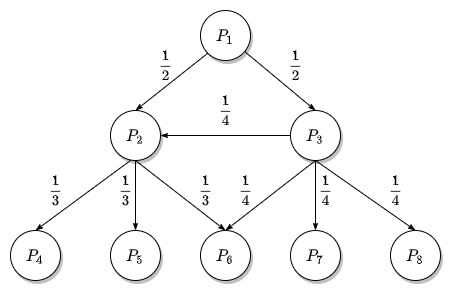
\includegraphics[width=0.5\textwidth]{./img/grafoprob}
\end{center}

Volvemos a considerar las mismas paginas web $P_1, P_2, \dots, P_n$ y $M$ la matriz de adyacencia del grafo, cuyas entradas $m_{ij}$ son $0$ y $1$. Llamamos $N_j$ al número de enlaces de la página $P_j$,  es decir al número de entradas de la columna $j$. Construimos una nueva matriz $M'$ a partir de la $M$ original sustituyendo cada $m_{ij}$ por
$$m'_{ij} = \frac{m_{ij}}{N_j} $$
La transformación sería la siguiente:

\begin{center}
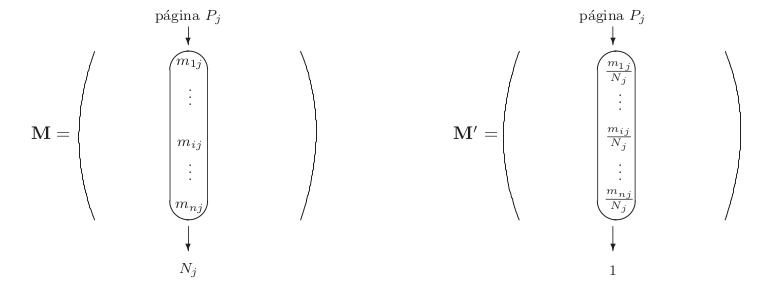
\includegraphics[width=0.9\textwidth]{./img/markov}
\end{center}

La nueva matriz $M'$ esta compuesta por números no negativos entre $0$ y $1$, a esta matriz así construida se le llama una matriz estocástica (o de Markov).

Con este modelo podemos conocer con que probabilidad estará el usuario en cada una de las páginas tras cada instante de tiempo. Por ejemplo, si el usuario parte de la página k-ésima $P_k$ para saber que probabilidad tiene de cambiar a cada uno de los posibles destinos solo tenemos que multiplicar la matriz $M'$ por el vector inicial. En este caso el vector inicial es un vector de ceros y un $1$ en la posición k-ésima, ya que sabemos que el usuario se encuentra en la página $P_k$ con una probabilidad del $100\%$.

Si multiplicamos $M'$ por el vector inicial, obtenemos:
$$\begin{pmatrix}
\cdots & \cdots & m'_{1k} & \cdots \\
\vdots & \ddots & \vdots & \vdots \\
\cdots & \cdtos & m'_{kk} & \cdots \\
\vdots & \vdots & \vdots & \ddots \\
\cdots & \cdots & m'_{nk} & \cdots \end{pmatrix} \begin{pmatrix}
0 \\
\vdots \\
1 \\
\vdots \\
0 \end{pmatrix} = \begin{pmatrix}
m'_{1k}\\
\vdots \\
m'_{kk} \\
\vdots \\
m'_{nk} \end{pmatrix}$$

Este vector resultante, cuyas entradas son o $0$ o $1/N_k$, describe con que probabilidad estará el usuario en cada una de las páginas tras una unidad de tiempo. Para saber con que probabilidad estará en cada uno de los posibles destinos dentro de dos unidades de tiempo solo debemos multiplicar el vector inicial por $(M')^2$, si lo queremos saber para dentro de tres unidades de tiempo lo multiplicaremos por $(M')^3$ y así sucesivamente.

La matriz $M'$ recibe el nombre de matriz de transición del sistema, ya que en cada entrada $m'_{ij}$ se refleja la probabilidad de pasar de la página $P_j$ a la página $P_i$. Y además las matrices que se corresponden con sus respectivas potencias también reflejan la probabilidad de pasar de $P_j$ a $P_i$ tras varios instantes de tiempo.

Sin embargo, podría ocurrir que alguna de las páginas no citaran a ninguna otra, es decir, que ese nodo del grafo no tuviera enlaces salientes. Esto se traduce en que en nuestra matriz $M'$ aparece una columna de ceros, por lo que esta matriz dejaría de ser estocástica y además el grafo del que partimos no estaría fuertemente conectado. Para solucionarlo se añade una probabilidad de transición a todos los vértices, es decir, añadimos la posibilidad de que el usuario se ``aburra'' y decida cambiar a otra página que no esté enlazada con la página en la que se encontraba. En términos matriciales se traduce en lo siguiente:

$$M'' = cM' + (1-c)\begin{pmatrix}
p_1 \\
\vdots \\
p_n \end{pmatrix} (1, \dots, 1)$$

\spanishdecimal{.}
Donde $p_1, \dots , p_n$ es una distribución de probabilidad y $c$ es un parámetro entre $0$ y $1$, el cual Google estima que se encuentra sobre $0,85$. La distribución de probabilidad a tomar puede ser una distribución uniforme que asigne una probabilidad de $p_i = 1/n$ a cada página, aunque también se podría elegir otras, ponderando unas páginas más que otras consiguiendo así búsquedas más personalizadas.

\newpage

\section{Pseudocódigo}
En esta sección comentaremos la estructura del algoritmo. Para implementarlo hemos separado el algoritmo en dos funciones. La primera función (\verb|pagerank|) se encarga de construir la matriz de adyacencia del grafo formado por todos los archivos y sus citas, además normaliza esta matriz por columnas para conseguir la matriz de transición del sistema y por último se le añade la el parámetro $c$ y la distribución de probabilidad uniforme como se comenta anteriormente, consiguiendo la matriz $M''$. La segunda función (\verb|metodopotencias|) tiene como objetivo calcular el vector propio de nuestra matriz $M''$, para ello se utiliza el método de las potencias.

\begin{algorithm}[H]
  \KwData{Vector que contiene todos los nodos (v)}
  \KwResult{Vector de pesos del PageRank (pg)}
  m = construyeMatrizAdyaencia(v)\;
  \For{i \in len(v)}{
    \If{ sum(m.T[i]) != 0}{
      m.T[i] = m.T[i] / sum(m.T[i])\;
    }
  }
  N = m[0].size()\;
  m\_seg = (C * m + (1 - C)/N)\;
  pg = metodopotencias(m\_seg, 100)\;
  \Return pg
\caption{pagerank}
\end{algorithm}

\begin{algorithm}[H]
  \KwData{M'' (m); Número de interaciones (num\_iter)}
  \KwResult{Vector de pesos del PageRank (v)}

  N = m[0].size()\;
  v = random(N, 1)\;
  v = v / max(v)\;
  \For{i $\in$ num\_iter}{
    v = m \cdot v
  }
  \Return v

\caption{metodopotencias}
\end{algorithm}

En el primer pseudocódigo \verb|m.T| se refiere a la traspuesta de \verb|m| y la constante \verb|C| tiene un valor de $0.85$ fijado previamente.

\newpage

\section{Ejemplos}
Para ilustrar como funciona el algoritmo del PageRank vamos a mostrar unos ejemplos. Comenzamos con el primer ejemplo, en este nos damos cuenta de que tanto $P_4$ como $P_5$ tienen dos enlaces entrantes, sin embargo, queda primero en la clasificación $P_5$, después $P_1$ y en tercer lugar $P_4$. Esto se debe a que una de los enlaces entrantes de $P_5$ es de $P_4$ una de las páginas con más enlaces. Recordemos que este algoritmo premia también si la página que cita es importante.

\underline{\textbf{Ejemplo 1}}

\begin{figure}[!ht]
  \begin{tabular}{*{2}{>{\centering\arraybackslash}b{\dimexpr0.5\linewidth-2\tabcolsep\relax}}}
  \centering
    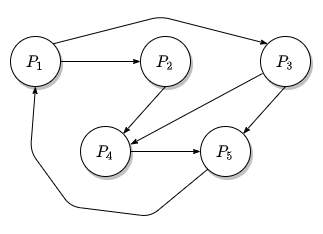
\includegraphics[scale=0.5]{./img/grafoej1}
    \caption{Grafo}
    &
      \renewcommand{\arraystretch}{1.3}
      \begin{tabular}{ccc}
         & Página & PageRank     \\ \hline
      1\textsuperscript{\underline{o}}} & $P_5$  & $0.26375504$ \\ \hline
      2\textsuperscript{\underline{o}}} & $P_1$  & $0.25419178$ \\ \hline
      3\textsuperscript{\underline{o}}} & $P_4$  & $0.20599017$ \\ \hline
      4\textsuperscript{\underline{o}}} & $P_2$  & $0.13803151$ \\ \hline
      5\textsuperscript{\underline{o}}} & $P_3$  & $0.13803151$ \\ \hline
      \end{tabular}\captionof{table}{Clasificación}
  \end{tabular}
\end{figure}

Añadimos al ejemplo dos páginas nuevas que también citan a $P_4$, sin embargo, esto no hace que $P_4$ se coloque en primera posición. Queda reflejado que el algoritmo da más puntuación a que la página tenga un enlace de una página importante que a una página con muchos enlaces.

\underline{\textbf{Ejemplo 2}}

\begin{figure}[!ht]
  \begin{tabular}{*{2}{>{\centering\arraybackslash}b{\dimexpr0.5\linewidth-2\tabcolsep\relax}}}
  \centering
    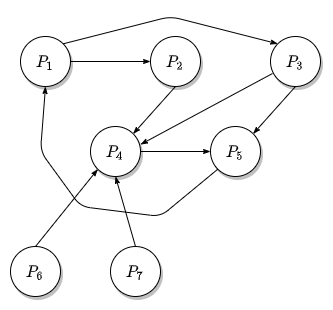
\includegraphics[scale=0.5]{./img/grafoej2}
    \caption{Grafo}
    &
      \renewcommand{\arraystretch}{1.3}
      \begin{tabular}{ccc}
        & Página & PageRank     \\ \hline
      1\textsuperscript{\underline{o}}} & $P_5$  & $0.2564552$  \\ \hline
      2\textsuperscript{\underline{o}}} & $P_1$  & $0.2394155$  \\ \hline
      3\textsuperscript{\underline{o}}} & $P_4$  & $0.21491184$ \\ \hline
      4\textsuperscript{\underline{o}}} & $P_2$  & $0.12318016$ \\ \hline
      5\textsuperscript{\underline{o}}} & $P_3$  & $0.12318016$ \\ \hline
      6\textsuperscript{\underline{o}}} & $P_7$  & $0.02142857$ \\ \hline
      7\textsuperscript{\underline{o}}} & $P_6$  & $0.02142857$ \\ \hline
      \end{tabular}\captionof{table}{Clasificación}
    \end{tabular}
\end{figure}

\newpage

Cambiamos la estrategía, en vez de añadir citas desde páginas nuevas hasta $P_4$ le añadimos una cita desde una de las páginas del grafo inicial, $P_1$, y obsevamos que tampoco conseguimos quitar a $P_5$ del primer puesto aunque la $P_4$ tenga más enlaces entrantes.

\underline{\textbf{Ejemplo 3}}

\begin{figure}[!ht]
  \begin{tabular}{*{2}{>{\centering\arraybackslash}b{\dimexpr0.5\linewidth-2\tabcolsep\relax}}}
  \centering
    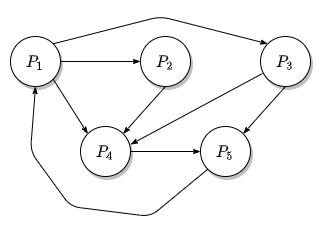
\includegraphics[scale=0.5]{./img/grafoej3}
    \caption{Grafo}
    &
      \renewcommand{\arraystretch}{1.3}
      \begin{tabular}{ccc}
        & Página & PageRank     \\ \hline
      1\textsuperscript{\underline{o}}} & $P_5$  & $0.27969961$ \\ \hline
      2\textsuperscript{\underline{o}}} & $P_1$  & $0.26774467$ \\ \hline
      3\textsuperscript{\underline{o}}} & $P_4$  & $0.24083375$ \\ \hline
      4\textsuperscript{\underline{o}}} & $P_2$  & $0.10586099$ \\ \hline
      5\textsuperscript{\underline{o}}} & $P_3$  & $0.10586099$ \\ \hline
      \end{tabular}\captionof{table}{Clasificación}
    \end{tabular}
\end{figure}

En el ejemplo anterior se comprueba la importancia del enlace saliente de $P_4$ capaz de colocar a una página en el primer puesto del ranking. De hecho si cambiamos este enlace y ponemos que salga de $P_4$ y llegue a $P_1$ convertimos a $P_1$ en la primera del ranking.

\underline{\textbf{Ejemplo 4}}

\begin{figure}[!ht]
  \begin{tabular}{*{2}{>{\centering\arraybackslash}b{\dimexpr0.5\linewidth-2\tabcolsep\relax}}}
  \centering
    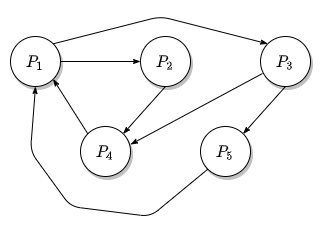
\includegraphics[scale=0.5]{./img/grafoej4}
    \caption{Grafo}
    &
      \renewcommand{\arraystretch}{1.3}
      \begin{tabular}{ccc}
        & Página & PageRank     \\ \hline
      1\textsuperscript{\underline{o}}} & $P_1$  & $0.32225461$ \\ \hline
      2\textsuperscript{\underline{o}}} & $P_4$  & $0.24287173$ \\ \hline
      3\textsuperscript{\underline{o}}} & $P_2$  & $0.16695821$ \\ \hline
      4\textsuperscript{\underline{o}}} & $P_3$  & $0.16695821$ \\ \hline
      5\textsuperscript{\underline{o}}} & $P_5$  & $0.10095724$ \\ \hline
      \end{tabular}\captionof{table}{Clasificación}
    \end{tabular}
\end{figure}

\newpage

Para conseguir que $P_4$, la página con más enlaces entrantes, se posicione la primera de la clasificación le quitamos los enlaces salientes.

\underline{\textbf{Ejemplo 5}}

\begin{figure}[!ht]
  \begin{tabular}{*{2}{>{\centering\arraybackslash}b{\dimexpr0.5\linewidth-2\tabcolsep\relax}}}
  \centering
    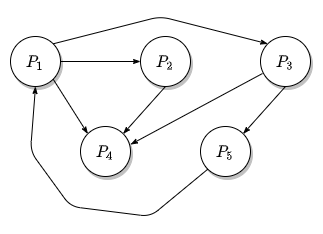
\includegraphics[scale=0.5]{./img/grafoej5}
    \caption{Grafo}
    &
      \renewcommand{\arraystretch}{1.3}
      \begin{tabular}{ccc}
        & Página & PageRank         \\ \hline
      1\textsuperscript{\underline{o}}} & $P_4$  & $2.79048247e-13$ \\ \hline
      2\textsuperscript{\underline{o}}} & $P_1$  & $2.47850051e-13$ \\ \hline
      3\textsuperscript{\underline{o}}} & $P_5$  & $1.86281319e-13$ \\ \hline
      4\textsuperscript{\underline{o}}} & $P_2$  & $1.31449230e-13$ \\ \hline
      5\textsuperscript{\underline{o}}} & $P_3$  & $1.31449230e-13$ \\ \hline
      \end{tabular}\captionof{table}{Clasificación}
    \end{tabular}
\end{figure}

Hemos visto que para el algoritmo puntúa más un enlace que sale de una página ``importante'' que muchos enlaces de páginas ``poco importantes''. En el siguiente ejemplo vemos que la página que más enlaces tiene es $P_3$ y la segunda $P_4$. Siguiendo el razonamiento anterior $P_3$ sería una página ``importante'' y su enlace valdría mucho, tanto que es capaz de colocar a cualquier página en primera posición. En este caso $P_3$ cita a $P_5$ convirtiéndola en una página ``importante'' y colocandola en primer lugar en la clasificación. Sin embargo, en este ejemplo añadimos un enlace desde $P_5$, página importante, a $P_3$ que también es importante, el resultado es un ajustado desempate (& $1.48851482e-06$ frente a $1.37701780e-06$) en el que resulta ganador $P_5$.

\underline{\textbf{Ejemplo 6}}

\begin{figure}[!ht]
  \begin{tabular}{*{2}{>{\centering\arraybackslash}b{\dimexpr0.5\linewidth-2\tabcolsep\relax}}}
  \centering
    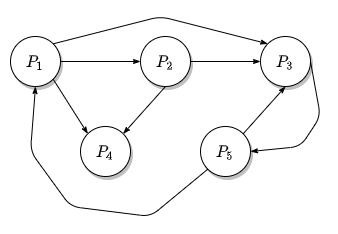
\includegraphics[scale=0.5]{./img/grafoej6}
    \caption{Grafo}
    &
      \renewcommand{\arraystretch}{1.3}
      \begin{tabular}{ccc}
        & Página & PageRank         \\ \hline
      1\textsuperscript{\underline{o}}} & $P_5$  & $1.48851482e-06$ \\ \hline
      2\textsuperscript{\underline{o}}} & $P_3$  & $1.37701780e-06$ \\ \hline
      3\textsuperscript{\underline{o}}} & $P_1$  & $8.80201594e-07$ \\ \hline
      4\textsuperscript{\underline{o}}} & $P_4$  & $6.61515329e-07$ \\ \hline
      5\textsuperscript{\underline{o}}} & $P_2$  & $4.46763904e-07$ \\ \hline
      \end{tabular}\captionof{table}{Clasificación}
    \end{tabular}
\end{figure}

Por último, nos preguntamos si las dos páginas tienen el mismo número de enlaces entrantes $P_3$ y $P_4$, quedando asi ``empatados'' y una de ellas no tiene enlaces salientes $P_4$. El resultado vuelve a ser ajustado, ganando $P_5$ (gracias al enlace desde $P_3$), en segundo puesto quedaría $P_3$ y en tercer lugar $P_4$. Por lo que no tener enlaces salientes solo te coloca en primer lugar si tienes más enlaces entrantes que las demás páginas.

\underline{\textbf{Ejemplo 7}}

\begin{figure}[!ht]
  \begin{tabular}{*{2}{>{\centering\arraybackslash}b{\dimexpr0.5\linewidth-2\tabcolsep\relax}}}
  \centering
    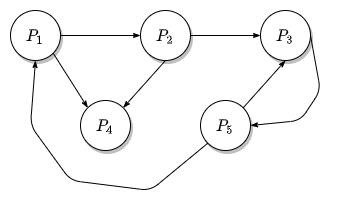
\includegraphics[scale=0.5]{./img/grafoej7}
    \caption{Grafo}
    &
      \renewcommand{\arraystretch}{1.3}
      \begin{tabular}{ccc}
        & Página & PageRank         \\ \hline
      1\textsuperscript{\underline{o}}} & $P_5$  & $7.66066766e-09$ \\ \hline
      2\textsuperscript{\underline{o}}} & $P_3$  & $6.60140578e-09$ \\ \hline
      3\textsuperscript{\underline{o}}} & $P_4$  & $5.18659092e-09$ \\ \hline
      4\textsuperscript{\underline{o}}} & $P_1$  & $4.86047008e-09$ \\ \hline
      5\textsuperscript{\underline{o}}} & $P_2$  & $3.44565523e-09$ \\ \hline
      \end{tabular}\captionof{table}{Clasificación}
    \end{tabular}
\end{figure}

\newpage

\section{Base de datos}

Para implementar el algoritmo de PageRank se ha utilizado la base de datos \textbf{PMSC-UGR} con
$26759991$ artículos. Esta base de datos basada en artículos científicos de MEDLINE/PubMed  pero
también utilizando SCopus herramienta de Elsevier. En PSMC-UGR se ha hecho el esfuerzo de
quitar las ambigüedades de los nombres de autores, para ello se ha establecido el ORCID, un número
que identifica a cada autor de manera unívoca. Cada archivo esta estructurado de la siguiente forma:
\begin{itemize}
\item \textit{PubMedID}. Es un identificador único del articulo proporcionado por PubMed.
\item \textit{Journal}. Es el nombre de la revista donde el artículo ha sido publicado.
\item \textit{ArticleTitle}. Es el título completo del artículo en inglés.
\item \textit{Abstract}. Resumen del artículo.
\item \textit{AuthorList}. Contiene información sobre los autores del artículo. Por cada uno podemos encontrar:
\begin{itemize}
\item \textit{LastName}. Contiene el apellido o el nombre único utilizado.
\item \textit{ForeName}. Contiene el resto del nombre.
\item \textit{Identifier}. Es un identificador único asociado con el nombre (ORCID).
\end{itemize}
\item \textit{MeshHeadingList}. Es un vocabulario controlado por NLM, encabezados de temas médicos (Mesh). Se utiliza para caracterizar el contenido del artículo utilizando descriptores de ese tesauro.
\item \textit{KeywordList}. Contiene términos controlados en palabras clave que también describen el contenido del artículo.
\end{itemize}

A estos datos se añaden las citas, el $66.78 \%$ de los artículos tienen alguna cita. La media de citas por artículo es de 7 y el total de citas es $3593931$. El numero de citas por articulo sigue una típica distribución \textit{ley de potencia} donde pocos artículos tienen muchas citas y muchos artículos tienen pocas citas. Por ejemplo, hay $116365$ artículos que tienen solo una cita y hay un artículo que tiene 713 citas.

Además esta base de datos ha sido procesada añadiendo las referencias de cada artículo, es decir, cada artículo conoce quien lo ha citado. Este dato no se utiliza en el algoritmo ya que por lo general no se suele conocer, cada artículo solo sabe que artículos ha citado y no llega a conocer los otro artículos que lo han citado. Sin embargo, se utilizará esta información para comprobar que son lógicos los resultados del Pagerank.


\section{Sistema basado en la información}
Un sistema de acceso a la información es un sistema dotado de un conjunto de técnicas para buscar, categorizar, modificar y acceder a la información que se encuentra en un sistema: base de datos, bibliotecas, archivos o internet.

\textbf{?`?` Poner esto en algún lado ??}

\textbf{Para borrar}
\begin{ndef}[Radio espectral]
Sea $A \in M_d(\mathbb{C})$ una matriz y $\sigma (A)$ el conjunto de valores propios de $A$. Definimos el radio espectral de una matriz, denotado por $\rho(A)$,  como:
$$\rho(A) = \max \{ | \lambda| : \lambda \in \sigma (A) \} $$
\end{ndef}

\begin{ndef}[Multiplicidad algebraica]
Sea $A \in M_d(\mathbb{C})$ una matriz cuadrada y $\lambda_1, \lambda_2, \dots, \lambda_r$ los distintos valores propios de $A$. LLamamos multiplicidad algebraica de $\lambda_i$, a la multiplicidad de $\lambda_i$ como raíz de $p(\lambda)$. A la multiplicidad algebraica de $\lambda_i$ la notamos como $m_i$ y se cumple que $m_1 + m_2 + \dots + m_r = d$.
\end{ndef}

\begin{ndef}[Multiplicidad geométrica]
Sea $A \in M_d(\mathbb{C})$ matriz cuadrada y $\lambda_1, \lambda_2, \dots, \lambda_r$ los distintos valores propios de $A$. LLamamos multiplicidad geométrica de $\lambda_i$ a la dimensión del subespacio propio $\mathscr{V}_\lambda_i$. A la multiplicidad geométrica de $\lambda_i$ la denotaremos como $\sigma_i$.
\end{ndef}

\begin{ndef}[Subespacio propio]
Sea $A \in M_d(\mathbb{C})$ una matriz cuadrada denotamos como $\mathscr{V}_\lambda$ al subespacio vectorial formado por vectores propios asociados al vector propio $\lamdba$. Además se cumple que  $\mathscr{V}_\lambda = Ker(A - \lambda I) = \{ v \in \mathbb{C}^d : Av = \lambda v \}$.
\end{ndef}

\begin{ndef}[Matrices semejantes]
Sean $A, B \in M_d(\mathbb{C})$ dos matrices cuadradas. Se dice que $A$ y $B$ son semejantes si existe una matriz $P \in M_d(\mathbb{C})$ invertible tal que:
$$A = P B P^{-1} $$
\end{ndef}

Sea $A \in M_n(\mathbb{C}), A > 0$, se cumplen las siguientes propiedades:
\begin{enumerate}
\item Si $\lambda \in \sigma(A)$ y $|\lambda| = \rho(A) \Rightarrow \lambda = \rho(A)$.
\end{enumerate}

\begin{proof}
Para demostrar que $\lambda_p$ es un valor propio dominante, veamos primero que es una raíz simple del polinomio característico, es decir que su multiplicidad algebraica sea $1$. Para ello llamamos $B = (I + A)^{n-1}$, la cual sabemos que es positiva por \ref{positiva}. Por \ref{funcionjordan} sabemos que $\lambda \in \sigma(A)$ si y solo si $(1 + \lambda)^{n-1} \in \sigma (B)$ y $alg mult_A(\lambda) = alg mult_B((1 + \lambda)^{n-1}).

Si llamamos $\mu = \rho(B)$, entonces tenemos:
$$\mu = \max_{\lambda \in \sigma(A)} |(1+ \lambda)|^{n-1} = \Big\{ \max_{\lambda \in \sigma(A)} |(1 + \lambda )| \Big\}^{n-1} = (1 + \lambda_p)^{n-1} $$

ya que si trasladamos el disco $|z| \leq \rho$ una unidad a la derecha obtenemos que el punto de módulo máximo del disco $|z+1| \leq \rho$ se alcanza en el punto $z = 1 + \rho$. \colorbox{yellow}{ Por lo tanto $alg\ mult_A(\lambda_p)=1$, ya que en otro caso $alg\ mult_B(\mu) > 1$, algo imposible} \colorbox{yellow}{ya que $B > 0$. ?`Por el teorema de Perron sobre B?}

Para ver que $A$ tiene un vector propio positivo asociado con $\lambda_p$, recordamos de \ref{vectorpropio} que existe un vector propio no negativo $\vec{x} \geq 0$ asociado con $\lambda_p$.
\colorbox{yellow}{Una consecuencia de \ref{radioespectral} es que si $(\lambda, \vec{x})$} \colorbox{yellow}{es un par propio de $A$, entonces $(f(\lambda),\vec{x})$ es un par propio de $f(A)$}:

Por \ref{radioespectral} sabemos que:
$$f(A) = \sum_{i = 1}^s \sum_{j = 0}^{k_i -1} \frac{f^{(j)}(\lambda_i)}{j!} (A - \lambda_iI)^j G_i$$
Supongamos que $\vec{x}$ es el valor propio de $\lambda_h$. Multiplicando por el vector $\vec{x}$ a ambos lados tenemos:
$$f(A)x = \left[\sum_{i = 1}^s \sum_{j = 0}^{k_i -1} \frac{f^{(j)}(\lambda_i)}{j!} (A - \lambda_iI)^j G_i \right] x = \left[ \sum_{j = 0}^{k_h -1} \frac{f^{(j)}(\lambda_h)}{j!} (A - \lambda_hI)^j \right] x = $$ $$ = \left[ \sum_{j = 0}^{k_h - 1} \frac{f^{(j)}(\lambda_h)}{j!} \left( \sum_{l = 1}^j {\from j \choose l} (-\lambda_h)^{j-l} A^l \right) \right]x = \sum_{j = 0}^{k_h - 1} \frac{f^{(j)}(\lambda_h)}{j!} \left( \sum_{l = 1}^j {\from j \choose l} (-\lambda_h)^{j-l} \lambda_h^l x \right) = $$ $$=  \left[ \sum_{j = 0}^{k_h - 1} \frac{f^{(j)}(\lambda_h)}{j!} \left( \sum_{l = 1}^j {\from j \choose l} (-\lambda_h)^{j-l} \lambda_h^l \right) \right]x = \left[\sum_{i = 1}^s \sum_{j = 0}^{k_i -1} \frac{f^{(j)}(\lambda_i)}{j!} (\lambda_h - \lambda_i)^j G_i \right] x = f(\lambda_h)x $$
\begin{center} \colorbox{yellow}{?`Es por lo que he puesto antes?} \end{center}
Por lo tanto que $(\lambda_p, \vec{x})$ sea un par propio para $A$ implica que $(\mu, \vec{x})$ sea un par propio para $B$. De \ref{nomasvalores} se deduce que $x$ será un múltiplo positivo del vector de Perron de $B$, por lo que $\vec{x}$ es positivo.

Además $\lambda_p$ es positivo, ya que de lo contrario $A\vec{x} = 0$, algo imposible ya que si $A \geq 0$ y $\vec{x} > 0$ entonces se da que $A\vec{x} > 0$. El mismo argumento que prueba \ref{nomasvalores}
demuestra el apartado 3.
\end{proof}


\newpage

\begin{thebibliography}{9}
\bibitem{algebralineal}
Carl D. Meyer
\textit{Matrix Analysis and Applied Linear Algebra}. Siam. 2000.

\bibitem{jordan}
Luis Merino y Evangelina Santos
\textit{Álgebra lineal con métodos elementales}. Paraninfo. 1999.

\bibitem{modelos}
Rafael Ortega Rios.
\textit{Modelos matemáticos}. Editorial Universidad de Granada. 2013.

\end{thebibliography}
%printbibliography

\end{document}
